\documentclass[12pt]{article}
\usepackage{arxiv}
\usepackage[utf8]{inputenc}
\usepackage[english, russian]{babel}
\usepackage[T1]{fontenc}
\usepackage{url}
\usepackage{booktabs}
\usepackage{amsfonts}
\usepackage{nicefrac}
\usepackage{microtype}
\usepackage{lipsum}
\usepackage{graphicx}
\usepackage{natbib}
\usepackage{doi}

\usepackage[utf8]{inputenc}
\usepackage{amsmath}
\usepackage{mathtools}




\title{Выбор интерпретируемых сверточных моделей глубокого обучения}

\author{ Тимур Мурадов\\
	МФТИ\\
	\And
	Олег Бахтеев \\
	МФТИ\\
	\And
	Константин Яковлев \\
	МФТИ\\
	\And
	Вадим Стрижов \\
	МФТИ\\
	%% \AND
	%% Coauthor \\
	%% Affiliation \\
	%% Address \\
	%% \texttt{email} \\
}
\date{}

\renewcommand{\undertitle}{}
\renewcommand{\headeright}{}
\renewcommand{\shorttitle}{Выбор интерпретируемых сверточных моделей глубокого обучения}

\hypersetup{
pdftitle={Выбор интерпретируемых сверточных моделей глубокого обучения},
pdfauthor={Тимур Мурадов},
pdfkeywords={Model interpretability \and Deep Learning \and OpenBox \and Convolutional neural networks},
}


\begin{document}
\maketitle

\begin{abstract}
	В статье рассматривается задача построения интерпретируемой сверточной нейронной сети. Под интерпретируемостью модели понимается выделение наиболее важных признаков и определение кластеров схожих объектов. Для повышения интерпретируемоси в статье вводится модификация метода OpenBox работающего с  кусочно-линейными нейронными сетями. В нём модель представляется в виде набора интерпретируемых линейных классификаторов. Каждый из них определен на выпуклом многограннике. Это позволяет классифицировать схожие объекты одним и тем же классификатором. Метод обобщается на работу с более широким классом нейронных сетей: сверточными нейронными сетями. Предлагается математически эквивалентная замена слоев свёрточной сети на линейные модели. Что  значительно повышает интепретируемость. Вычислительный эксперимент проводится на выборках изображений рукописных цифр MNIST и изображений CIFAR-10.
\end{abstract}


\keywords{Model interpretability \and Deep Learning \and OpenBox \and Convolutional neural networks}

\section{Introduction}
В данном исследовании стоит задача повышения интерпретируемости модели, где под интерпретируемостью понимается простота выделения важных признаков на выборке данных и классификация близких объектов одним и тем же классификатором.

Проблемой является в целом высокая сложность интерпретации сверточных нейронных сетей, требующая комплексного подхода. На данный момент существует множество различных решений проблемы интерпретации \cite{ribeiro2016why, Lundberg2017aunified, chu2019exact} . В статье \cite{ribeiro2016why} описан метод \textbf{LIME}, предлагащий линейную апроксимацию предсказаний модели в некоторой небольшой окрестности вокруг объектов из тестовой выборки. Такой подход позволяет получить простую для интерпретации модель без использования информации о строении модели изнутри \textquotedblleft model-agnostic\textquotedblright. Но он весьма неустойчив к выбросам и сильно зависим от точности апроксимации. В статье \cite{Lundberg2017aunified} предлагается подход \textbf{SHAP}, заключающийся в рассмотрении вклада каждого признака в работу модели. Таким образом удается выделять даже скрытые, но значимые признаки. Однако применимость данного подхода ограничена ввиду высоких вычислительных затрат: требуется многократное обучение модели, и он весьма зависим от выборки данных. Ещё один подход к интерпретации \textbf{OpenBox}, описываемый в статье \cite{chu2019exact} предлагает построение математически эквивалентных линейных моделей для линейных нейронных сетей. Он показал более высокую эффективность по сравнению с \textbf{LIME} и весьма перспективен для дальнейшей работы.

В данной работе предлагается адаптация метода \textbf{OpenBox} для работы со свёрточными нейронными сетями: математически эквивалентно представить в виде линейных моделей такие слои как свёртка, пулинг и нормализация. И сравнение с альтернативными методами интепретации CNN.

Для анализа качества предложенного метода проводится вычислительный эксперимент на выборке изображений Fashion-MNIST \citep{fashionmnist}.



\section{Problem Definition}
\label{sec:headings}

Задана выборка $\mathbf{x} \in \mathbf{X}$ двумерные трехканальные изображения. $\mathbf{X} \in \{1, 2, ... k\}$, заданное конечное множество классов.

Рассматривается задача построения модели глубокого обучения для задачи классификации.

Модель $\mathbf{f}(\mathbf{X}, \mathbf{w})$ --- сверточная нейронная сеть, для краткости CNN, это суперпозиция подмоделей $\mathbf{f_1} \circ \mathbf{f_2} \dots \mathbf{f_n}$.

Функции $\mathbf{f_i}$ --- слои нейронной сети, это одни из функций: линейные $\mathbf{f_i} = \mathbf{w_0} + \Sigma \mathbf{w_i} * \mathbf{x_i}$, свертки $S(i,j) = (K * I)(i,j) = \Sigma_m \Sigma_n I(i + m, j + n)K(m, n)$, батч-нормы $\hat{x_i^{(k)}} = \frac{x_i^{(k)} - E(x_i^{(k)})}{\sqrt{D(x_i^{(k)})}}$ или пулинги.

$\mathbf{f}(\mathbf{X}, \mathbf{w})$ оптимизирует функцию кросс энтропии $\mathcal{L}$, $\mathbf{g}$ --- функция softmax.

$$\mathbf{g}(\mathbf{x})_i = \frac{e^{\mathbf{x_i}}}{\Sigma_j e^{\mathbf{x_j}}}$$
$$\mathcal{L} = -\Sigma_i \log \mathbf{g}(\mathbf{x})_i \to \max$$

Кроме задачи оптимизации модель также должна удовлетворять следующим требованиям к итерпретируемости: $\textbf{Точность}$ и $\textbf{Консистентность}$.
\begin{itemize}
    \item \textbf{Точность}:
    Математическая эквивалентность.
    $$\mathbf{f}(\mathbf{X}, \mathbf{w}) = \mathbf{f_{true}}(\mathbf{X}, \mathbf{w})$$
    \item \textbf{Консистентность}:
    Близкие интерпретации для близких объектов выборки. $$\mathbf{x_i} \approx \mathbf{x_j} \Longrightarrow \mathbf{f}(\mathbf{x_i}, \mathbf{w}) \approx \mathbf{f}(\mathbf{x_j}, \mathbf{w})$$
\end{itemize}


\section{Theory}

\newtheorem{hypothesis}{Hypothesis}
\begin{hypothesis}
Слои сверточной нейронной сети: линейные, свертки, батч-нормализации, пулинги --- это линейные операции.
\end{hypothesis}

\begin{proof}
\begin{itemize}
    \item Линейный слой линеен по определению. 
    $$\mathbf{f_i} = \mathbf{w_0} + \Sigma \mathbf{w_i} * \mathbf{x_i}$$
    \item Свертка представима как линейная операция, если расписать её в специфичном виде как произведение матрицы входного изображения на матрицу с весами фильтра.
    \item Пулинг на максимум представим как взаимодействие фильтра на изображение как на политоп.
    \item Батч нормализация представима в виде скалярного произведения, применная поэлементно к каждому изображению.
\end{itemize}
\end{proof}

\section{Computational experiment}

Цель эксперимента: проверить работоспособность базового метода LIME \cite{ribeiro2016why} и сравнить качество работы с предлагаемой альтернативой OpenBox \cite{chu2019exact}. Критерием качества рассматривается точность предсказания класса объектов. Отличие $P(i)$ для метода от истинной вероятности, полученной из классификатора, где $P$ - вероятность принадлежности к классу, $i$ - индекс рассматриваемого объекта.

\section{Our setup}


Строим CNN и при помощи метода LIME \cite{ribeiro2016why} получаем интерпретации признаков модели.

\subsection{Data}

  Fashion-MNIST датасет содержащий 60000 изображений в train и 10000 изображений в test из 10 различных классов. Каждое изображение имеет разрешение 28*28 пикселей  \citep{fashionmnist}.

\subsection{Configuration of algorithm run}

Считаем точность предсказаний и расстояние между признаками, полученные при помощи алгоритма LIME \cite{ribeiro2016why}.

\begin{figure}
  \subfloat{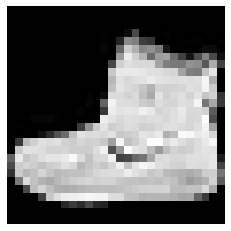
\includegraphics[width=0.5\textwidth]{example.png}}
  \subfloat{\includegraphics[width=0.5\textwidth]{example_Lime.png}}
 \caption{Lime features decision}
  \label{fig:1}
\end{figure}

\subsection{Preliminary report}

\begin{figure}
\subfloat{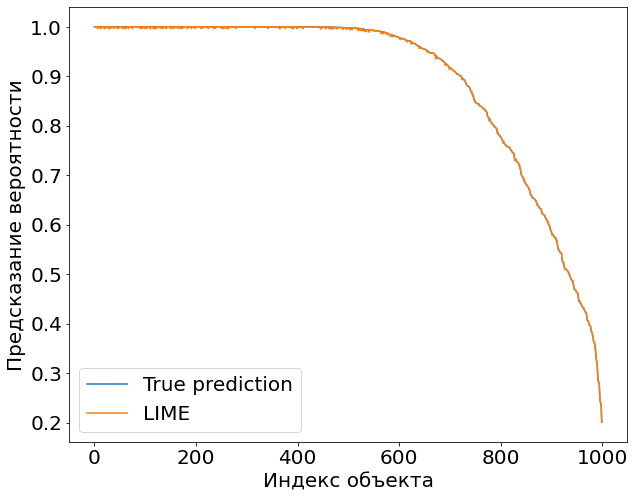
\includegraphics[width=0.70\textwidth]{lime_and_true.png}}
\caption{Lime accuracy}
\label{fig:image}
\end{figure}

\newpage

\subsection{Error analysis}

Рассмотриваем простейшую модель сверточной нейронной сети и адаптируем методу OpenBox \cite{chu2019exact}, далее сравниваем полученные результаты с приминением базового метода LIME \cite{ribeiro2016why}.

\newpage

\bibliographystyle{unsrt}
\bibliography{ref}

\end{document}